$S_X$ refers to the set of all permutations on the set $X$. That is, the elements of $S_X$ are bijections from $X$ to itself. $S_n$ refers to when $X=\set{1,2,\ldots,n}.$

Let $n=5$. How many elements are in $S_5$? $5!=120$. Why? Given a $\sigma \in S_5$, we have $5$ choices for $\sigma(1)$, 4 for $\sigma(2),...$ so there are $5\cdot 4 \cdot 3 \cdot 2 \cdot 1=5! = 120$ choices for $\sigma$. In general, there $n!$ elements in $S_n$.

$S_5:$ how many cycles of length $5$ are in $S_5$?

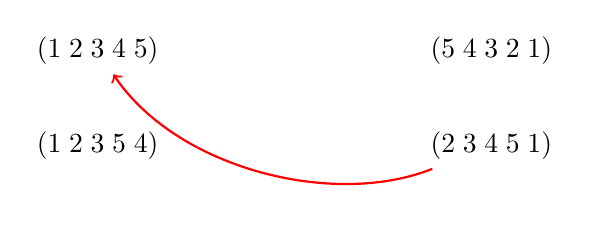
\begin{tikzpicture}[baseline=(current bounding box.center)]
\node (a) at (0,0) {$(1\;2\;3\;4\;5)$};
\node (b) at (5,0) {$(5\;4\;3\;2\;1)$};
\node (c) at (0,-1.2) {$(1\;2\;3\;5\;4)$};
\node (d) at (5,-1.2) {$\cancel{(2\;3\;4\;5\;1)}$};
\draw[->, red, thick] (d) .. controls (3,-2) and (1,-1.5) .. (a);
\end{tikzpicture} 

$\vdots$

There are $5!$ ways of filling in a blank 5-cycle. However, each 5-cycle is represented 5 ways, so we divide by 5. Thus there are $\frac{5!}{5} = 4! = 24$ distinct 5-cycles in $S_5$.How many
\begin{align*}
    \text{4 cycles? } & \frac{5\cdot4\cdot3\cdot2}{4} = 30 \\
    \text{3 cycles? } & \frac{5\cdot4\cdot3}{3} = 20 \\
    \text{2 cycles? } & \frac{5\cdot4}{2} = 10 \\
    \text{1 cycles? } & \frac{5}{1} = 5
\end{align*}

How many distinct $r$-cycles $r \leq n$ are there in $S_n$? $\frac{n!}{r(n-r)!}$
$$\frac{n\cdot(n-1)\cdot(n-2)\cdots(n-r+1)}{r!}$$

How many distinct elements of the form $(\_ \_)(\_ \_ \_)$ disjoint in $S_5$?
$$\frac{5\cdot4}{2} \cdot \frac{3\cdot2\cdot1}{3} = 20$$

How many of the form $(\_ \_)(\_ \_)$?
$$\frac{\frac{5\cdot4}{2} \cdot \frac{3\cdot2}{2}}{2} = \frac{30}{2}=15$$

How many distinct elements of the form $(\_ \_)(\_ \_ \_)$ in $S_n$?
$$\frac{n\cdot(n-1)}{2} \cdot \frac{(n-2)(n-3)(n-4)}{3}$$

How many distinct elements of the form $(\_ \_)(\_ \_)$ in $S_n$?
$$\frac{\frac{n\cdot(n-1)}{2} \cdot \frac{(n-2)(n-3)}{2}}{2}$$

\begin{definition}[Field] \leavevmode \\
    $(F, +, \cdot)$ is a field if
    \begin{enumerate}
        \item $(F, +)$ is an abelian group with identity $0$
        \item $(F\setminus\set{0}, \cdot)$ is an abelian group with identity $1$
        \item Left and right distributive laws hold
    \end{enumerate}
\end{definition}

The following are groups:
\begin{align*}
    GL_n(F) &= \set{\text{all $n\times n$ matrices with entries in $F$ and with non-zero determinants}} \\
    SL_n(F) &= \set{\text{all $n\times n$ matrices with entries in $F$ and with determinant $1$}}
\end{align*}